\documentclass{ximera}

%% You can put user macros here
%% However, you cannot make new environments

\listfiles

\graphicspath{{./}{firstExample/}{secondExample/}}

\usepackage{tikz}
\usepackage{tkz-euclide}
\usepackage{tikz-3dplot}
\usepackage{tikz-cd}
\usetikzlibrary{shapes.geometric}
\usetikzlibrary{arrows}
\usetikzlibrary{decorations.pathmorphing,patterns}
\usetkzobj{all}
\pgfplotsset{compat=1.13} % prevents compile error.

\renewcommand{\vec}[1]{\mathbf{#1}}
\newcommand{\RR}{\mathbb{R}}
\newcommand{\dfn}{\textit}
\newcommand{\dotp}{\cdot}
\newcommand{\id}{\text{id}}
\newcommand\norm[1]{\left\lVert#1\right\rVert}
 
\newtheorem{general}{Generalization}
\newtheorem{initprob}{Exploration Problem}

\tikzstyle geometryDiagrams=[ultra thick,color=blue!50!black]

\usepackage{mathtools}

\title{Introduction to Systems of Differential Equations}%\label{Module 7-ADEF}


\begin{document}

\begin{abstract}

\end{abstract}

\maketitle

\section*{Introduction to Systems of Differential Equations}

Many physical situations are modelled by systems of $n$ differential equations
in $n$ unknown functions, where $n\geq 2$. The next three examples
illustrate physical problems that lead to systems of differential
equations. In these examples and throughout this chapter we'll
denote the independent variable by $t$.

\begin{example}\label{example:10.1.1}  
Tanks $T_1$ and $T_2$ contain 100 gallons and 300 gallons of salt
solutions, respectively. Salt solutions are simultaneously added to
both tanks from external sources, pumped from each tank to the other,
and drained from both tanks (see the figure below). 

\begin{image}
 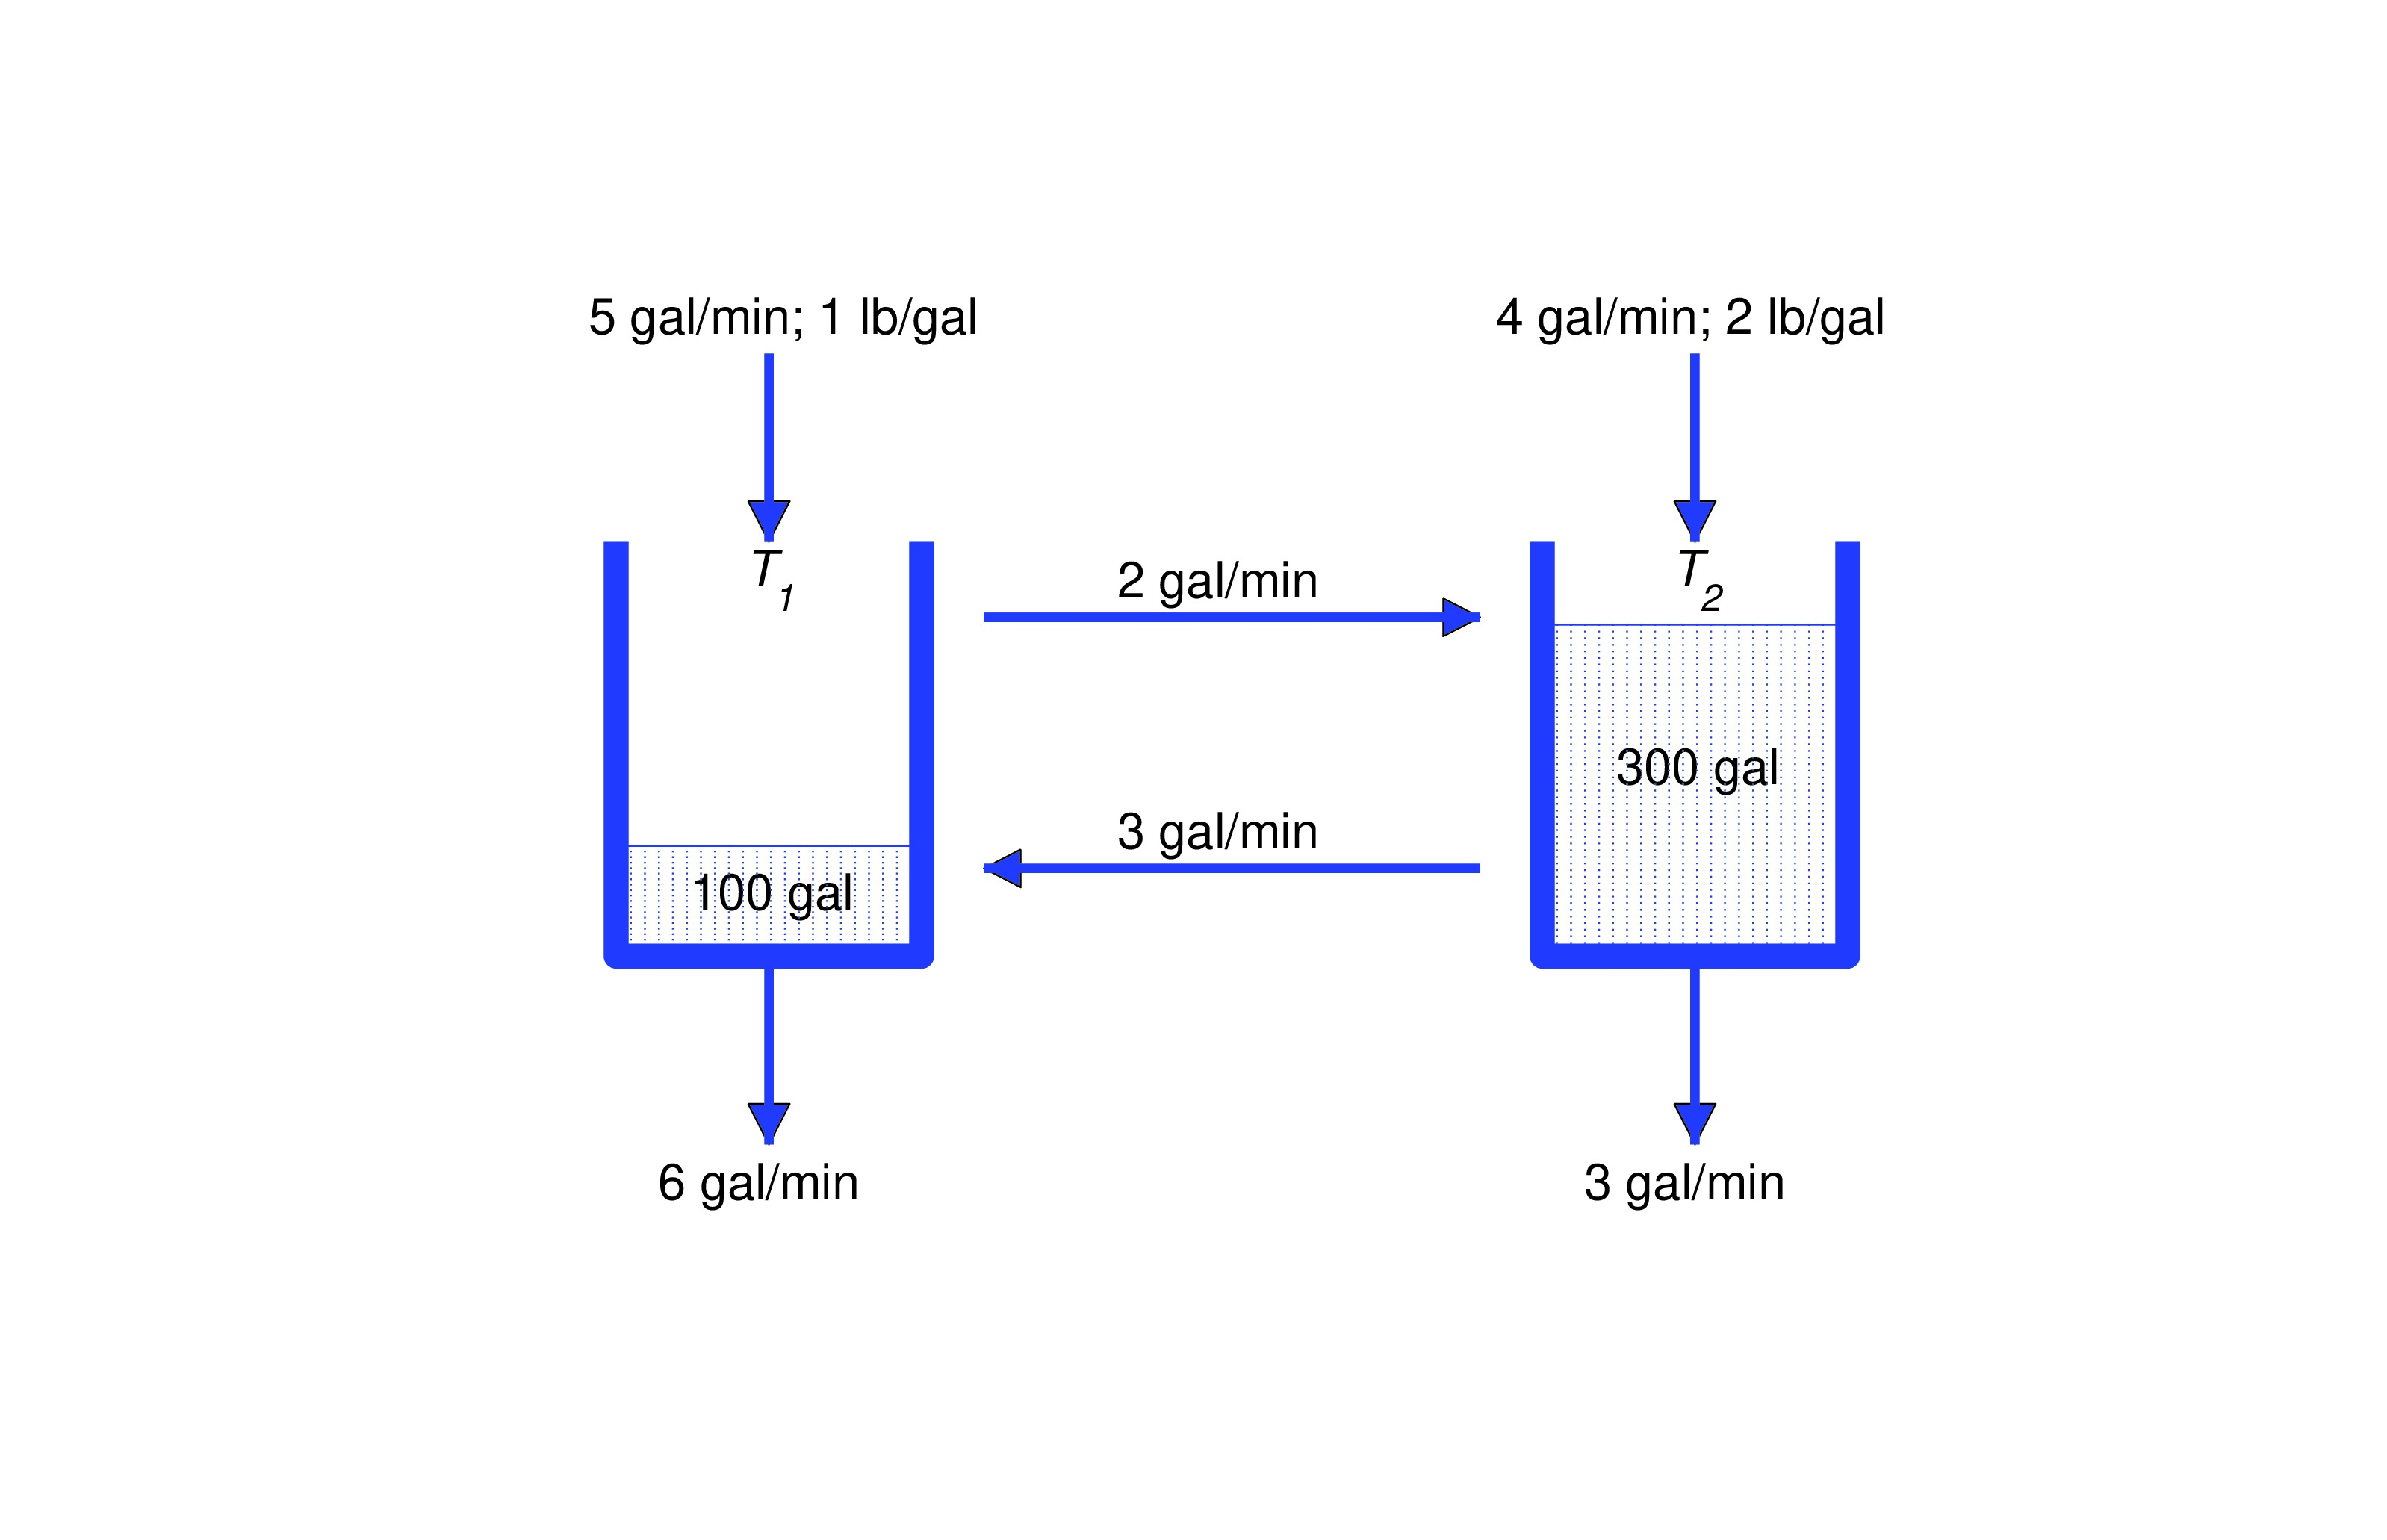
\includegraphics[height=1.5in]{fig100101.jpg} 
\end{image}

A solution with
$1$ pound of salt per gallon is pumped into $T_1$ from an external source
at $5$~gal/min, and a solution with $2$ pounds of salt per gallon is
pumped into $T_2$ from an external source at $4$~gal/min. The solution
from $T_1$ is pumped into $T_2$ at 2 gal/min, and the solution from
$T_2$ is pumped into $T_1$ at $3$ gal/min. $T_1$ is drained at $6$~gal/min
and $T_2$ is drained at 3~gal/min. Let $Q_1(t)$ and $Q_2(t)$ be the
number of pounds of salt in $T_1$ and $T_2$, respectively, at time
$t>0$. Derive a system of differential equations for $Q_1$ and $Q_2$.
Assume that both mixtures are well stirred.

\begin{explanation}
As in Section~4.2, let \dfn{rate in} and \dfn{rate
out} denote the rates (lb/min) at which salt enters and leaves a tank;
thus,
\begin{eqnarray*}
Q_1'&=&(\mbox{rate in})_1-(\mbox{rate out})_1,\\
Q_2'&=&(\mbox{rate in})_2-(\mbox{rate out})_2
\end{eqnarray*}
Note that the volumes of the solutions in $T_1$ and $T_2$
remain constant at 100~gallons and 300~gallons, respectively.

$T_1$ receives salt from the external source at the rate of
$$
\mbox{(1 lb/gal) }\times\mbox{ (5~gal/min)}=\mbox{ 5 lb/min},
$$
and from $T_2$ at the rate of
$$
\mbox{(lb/gal in }T_2)\times\mbox{ (3~gal/min)
}=\frac{1}{300}Q_2\times3\\=\frac{1}{100}Q_2 \mbox{ lb/min}.
$$
Therefore
\begin{equation} \label{eq:10.1.1}
\mbox{(rate in)}_1= 5+\frac{1}{100}Q_2.
\end{equation}
Solution leaves $T_1$  at the rate of 8~gal/min, since 6~gal/min are
drained and 2~gal/min are pumped to $T_2$; hence,
\begin{equation} \label{eq:10.1.2}
(\mbox{rate out})_1=(\mbox{ lb/gal in T}_1)\times \mbox{(8~gal/min) }
=\frac{1}{100}Q_1\times8=\frac{2}{25}Q_1.
\end{equation}
Eqns.~\eqref{eq:10.1.1} and \eqref{eq:10.1.2}  imply that
\begin{equation} \label{eq:10.1.3}
Q_1'=5+\frac{1}{100}Q_2-\frac{2}{25}Q_1.
\end{equation}

$T_2$ receives salt from the external source at the rate of
$$
\mbox{(2 lb/gal) }\times\mbox{ (4~gal/min)}=\mbox{ 8 lb/min},
$$
and from $T_1$ at the rate of
$$
\mbox{(lb/gal in }T_1)\times\mbox{ (2~gal/min)
}=\frac{1}{100}Q_1\times 2\\=\frac{1}{50}Q_1 \mbox{ lb/min}.
$$
Therefore
\begin{equation} \label{eq:10.1.4}
\mbox{(rate in)}_2= 8+\frac{1}{50}Q_1.
\end{equation}
Solution leaves $T_2$  at the rate of $6$~gal/min, since $3$~gal/min are
drained and $3$~gal/min are pumped to $T_1$; hence,
\begin{equation} \label{eq:10.1.5}
(\mbox{rate out})_2=(\mbox{ lb/gal in T}_2)\times \mbox{(6~gal/min) }
=\frac{1}{300}Q_2\times6=\frac{1}{50}Q_2.
\end{equation}
Eqns.~\eqref{eq:10.1.4} and \eqref{eq:10.1.5} imply that
\begin{equation} \label{eq:10.1.6}
Q_2'=8+\frac{1}{50}Q_1-\frac{1}{50}Q_2.
\end{equation}

We say that \eqref{eq:10.1.3} and \eqref{eq:10.1.6}  form a \dfn{system of two
first order equations in two unknowns}, and write them together as
\begin{eqnarray*}
Q_1'&=&5-\frac{2}{25}Q_1+\frac{1}{100}Q_2\\
Q_2'&=&8+\frac{1}{50}Q_1-\frac{1}{50}Q_2
\end{eqnarray*}

\end{explanation}
\end{example}


\begin{example}\label{example:10.1.2}
A mass $m_1$ is suspended from a rigid support on a spring $S_1$ and a
second mass $m_2$ is suspended from the first on a spring $S_2$
(see the figure below). 

\begin{image}
 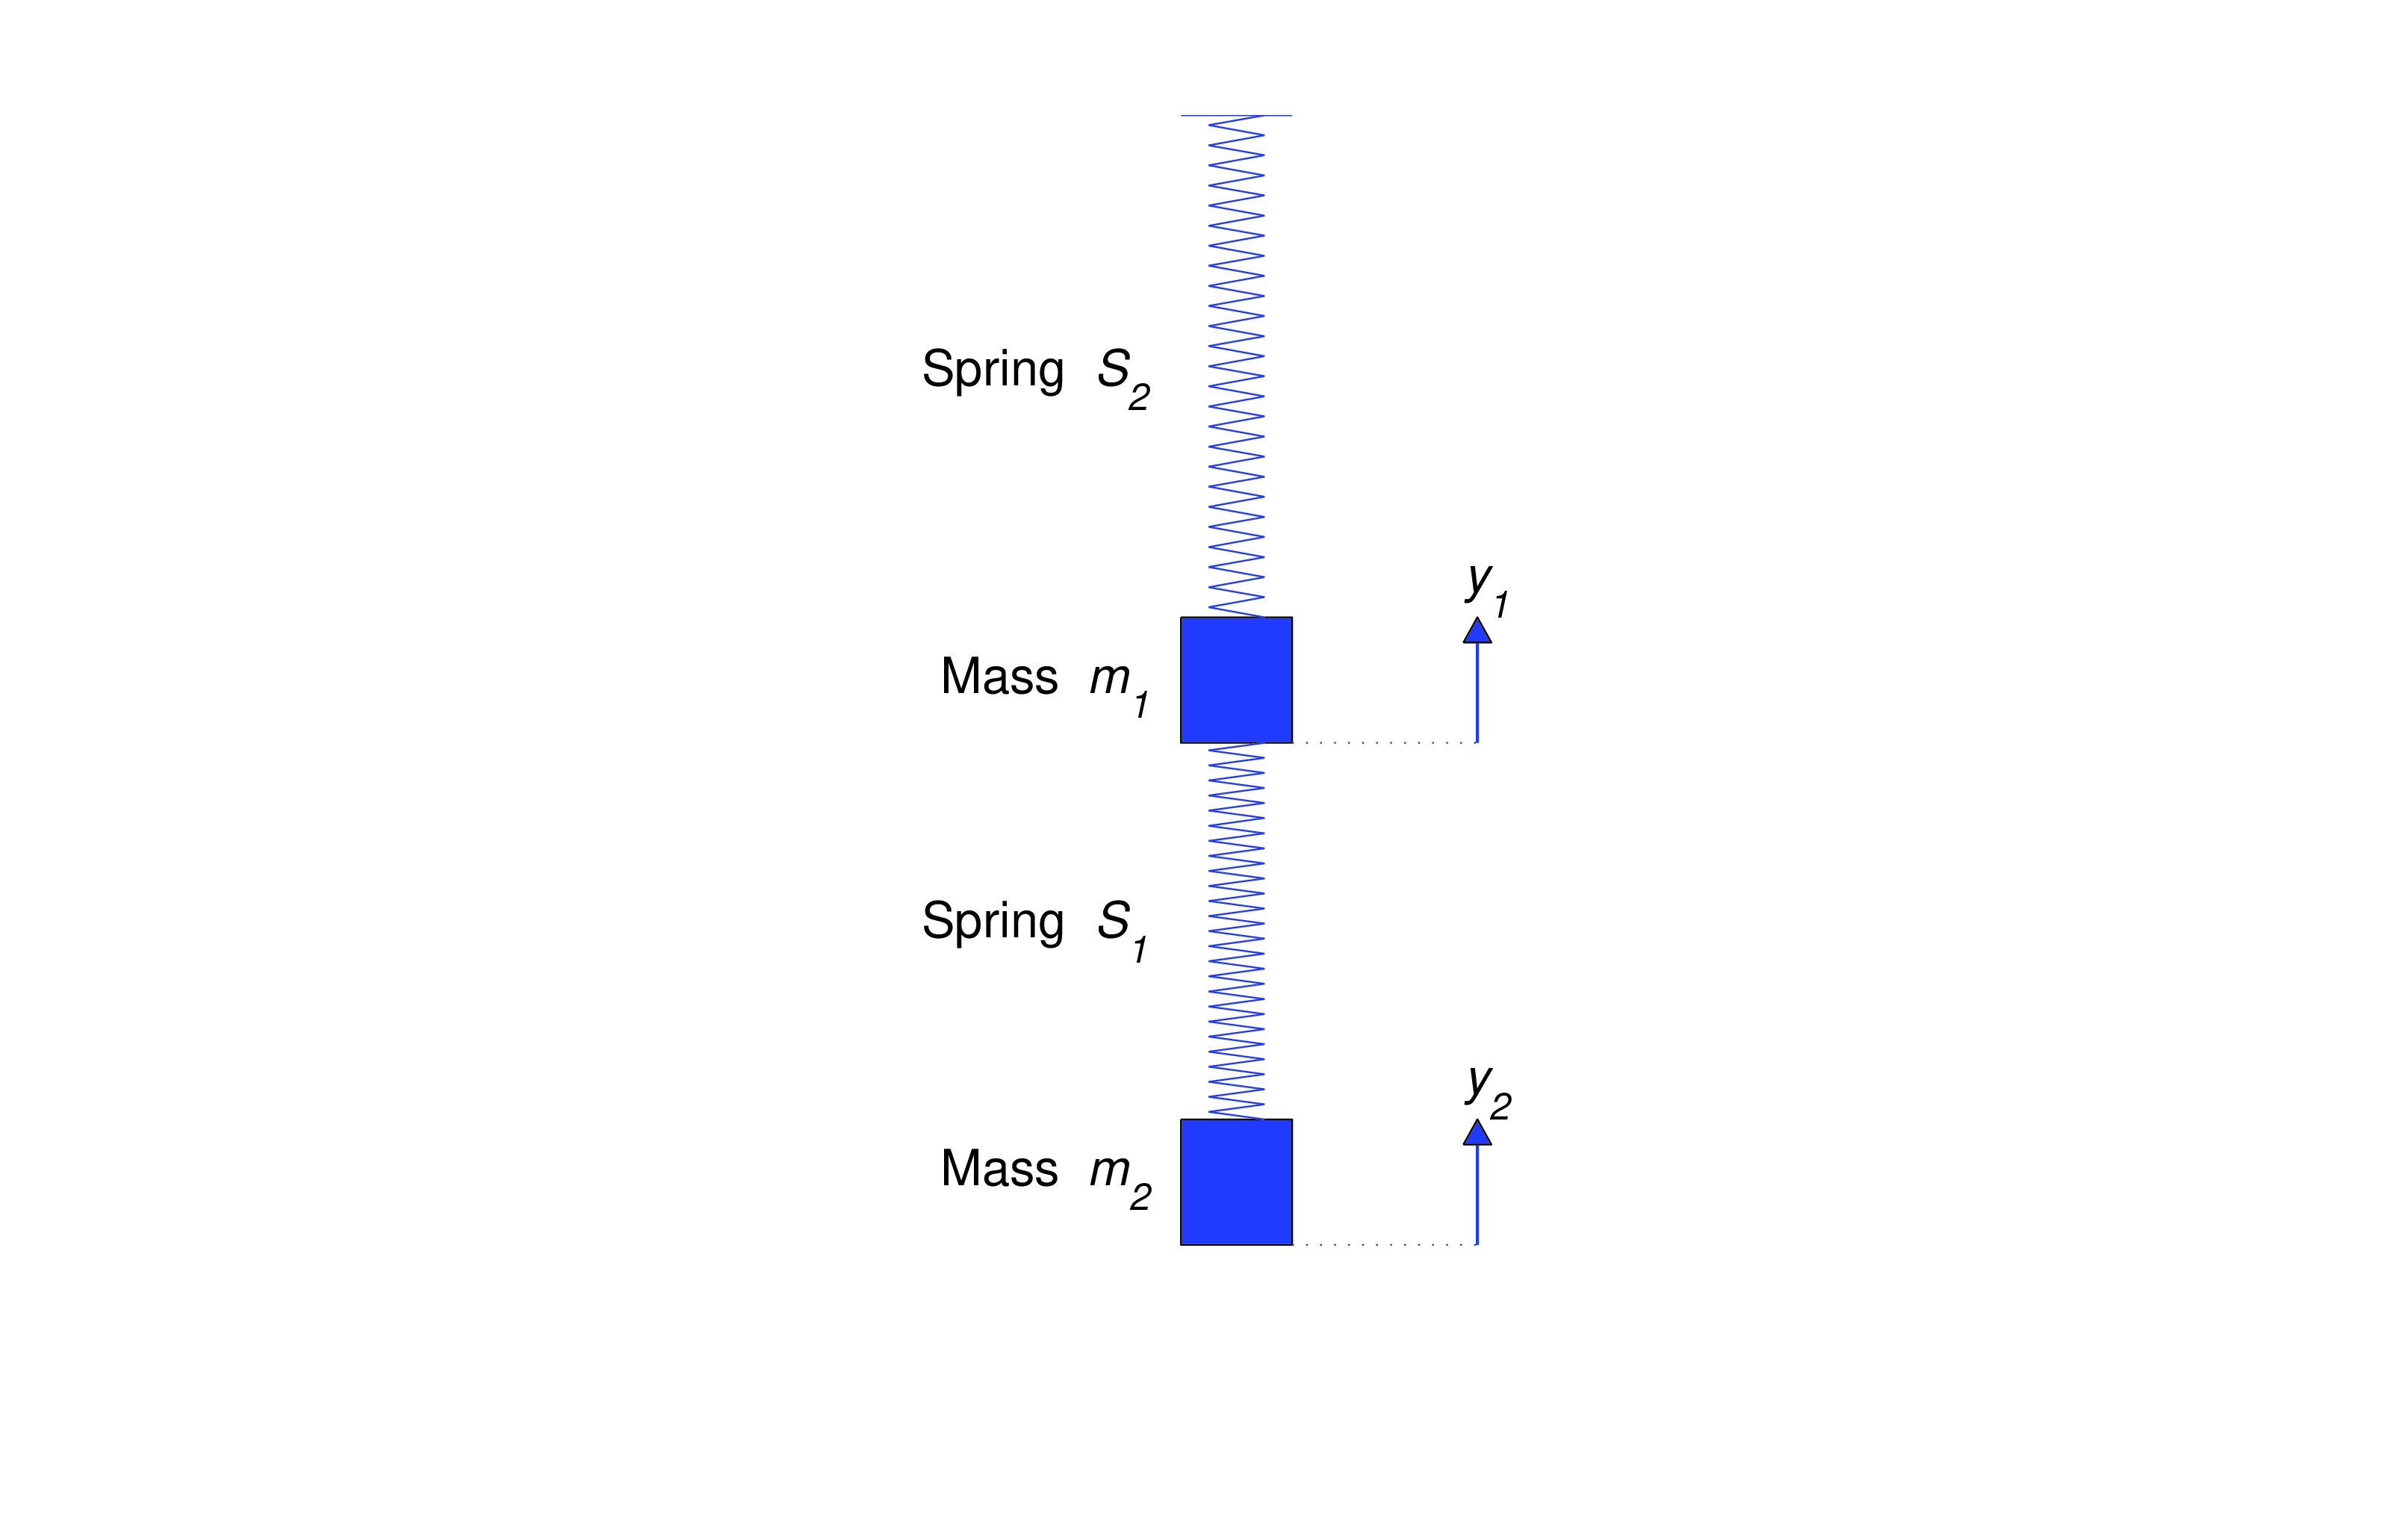
\includegraphics[height=1.5in]{fig100102.jpg} 
\end{image}

The springs obey Hooke's law, with spring
constants $k_1$ and $k_2$. Internal friction causes the springs to
exert damping forces proportional to the rates of change of their
lengths, with damping constants $c_1$ and $c_2$. Let $y_1=y_1(t)$ and
$y_2=y_2(t)$ be the displacements of the two masses from their
equilibrium positions at time $t$, measured positive upward.
 Derive a system of differential equations
for $y_1$ and $y_2$, assuming that the masses of the springs are
negligible and that vertical external forces $F_1$ and $F_2$ also act
on the objects.


\begin{explanation}
In equilibrium, $S_1$ supports both $m_1$ and $m_2$ and $S_2$ supports
only $m_2$. Therefore, if $\Delta\ell_1$ and $\Delta\ell_2$ are the
elongations of the springs in equilibrium then
\begin{equation} \label{eq:10.1.7}
(m_1+m_2)g=k_1\Delta\ell_1\quad\mbox{and}\quad m_2g=k_2\Delta\ell_2.
\end{equation}

Let $H_1$ be the Hooke's law force acting on $m_1$, and let $D_1$ be
the damping force on $m_1$. Similarly, let $H_2$ and $D_2$ be the
Hooke's law and damping forces acting on $m_2$. According to Newton's
second law of motion,
\begin{equation} \label{eq:10.1.8}
\begin{array}{ccl}
m_1y_1''=-m_1g+H_1+D_1+F_1,\\
m_2y_2''=-m_2g+H_2+D_2+F_2.
\end{array}
\end{equation}
When the displacements are $y_1$ and $y_2$, the change in length of
$S_1$ is $-y_1+\Delta\ell_1$ and the change in length of $S_2$ is
$-y_2+y_1+\Delta\ell_2$. Both springs exert Hooke's law forces on $m_1$,
while only $S_2$ exerts a Hooke's law force on $m_2$. These forces are
in directions that tend to restore the springs to their natural
lengths. Therefore
\begin{equation} \label{eq:10.1.9}
H_1=k_1(-y_1+\Delta\ell_1)-k_2(-y_2+y_1+\Delta\ell_2)\quad\mbox{and}\quad H_2=k_2(-y_2+y_1+\Delta\ell_2).
\end{equation}
When the velocities are $y_1'$ and $y_2'$,  $S_1$ and $S_2$ are
changing length at the rates $-y_1'$ and $-y_2'+y_1'$, respectively.
Both springs exert damping forces on $m_1$, while only $S_2$ exerts a
damping force on $m_2$. Since the force due to damping exerted by a
spring is proportional to the rate of change of length of the spring
and in a direction that opposes the change, it follows that
\begin{equation} \label{eq:10.1.10}
D_1=-c_1y_1'+c_2(y_2'-y_1')\quad\mbox{and}\quad
D_2=-c_2(y_2'-y_1').
\end{equation}

From \eqref{eq:10.1.8}, \eqref{eq:10.1.9}, and \eqref{eq:10.1.10},
\begin{equation} \label{eq:10.1.11}
\begin{array}{ccl}
m_1y_1''&=&-m_1g+k_1(-y_1+\Delta\ell_1)-k_2(-y_2+y_1+\Delta\ell_2)\\
  & &-c_1y_1'+c_2(y_2'-y_1')+F_1\\
&=&-(m_1g-k_1\Delta\ell_1+k_2\Delta\ell_2)-k_1y_1+k_2(y_2-y_1)\\
& &-c_1y_1'+c_2(y_2'-y_1')+F_1
\end{array}
\end{equation}
and
\begin{equation} \label{eq:10.1.12}
\begin{array}{ccl}
m_2y_2''&=&-m_2g+k_2(-y_2+y_1+\Delta\ell_2)-c_2(y_2'-y_1')+F_2\\
&=&-(m_2g-k_2\Delta\ell_2)-k_2(y_2-y_1)-c_2(y_2'-y_1')+F_2.
\end{array}
\end{equation}
From \eqref{eq:10.1.7},
$$
m_1g-k_1\Delta\ell_1+k_2\Delta\ell_2=-m_2g+k_2\Delta\ell_2=0.
$$
Therefore we can rewrite \eqref{eq:10.1.11} and \eqref{eq:10.1.12}
as
\begin{eqnarray*}
m_1y_1''&=&-(c_1+c_2)y_1'+c_2y_2'-(k_1+k_2)y_1+k_2y_2+F_1\\
m_2y_2''&=&c_2y_1'-c_2y_2'+k_2y_1-k_2y_2+F_2.
\end{eqnarray*}
\end{explanation}
\end{example}

\begin{example}\label{example:10.1.3}
Let $\vec{X}=\vec{X}(t)=x(t)\,\vec{i}+y(t)\,\vec{j}+z(t)\,\vec{k}$ be
the position vector at time $t$ of an object with mass $m$, relative
to a rectangular coordinate system with origin at Earth's center
(see the figure below). 

\begin{image}
 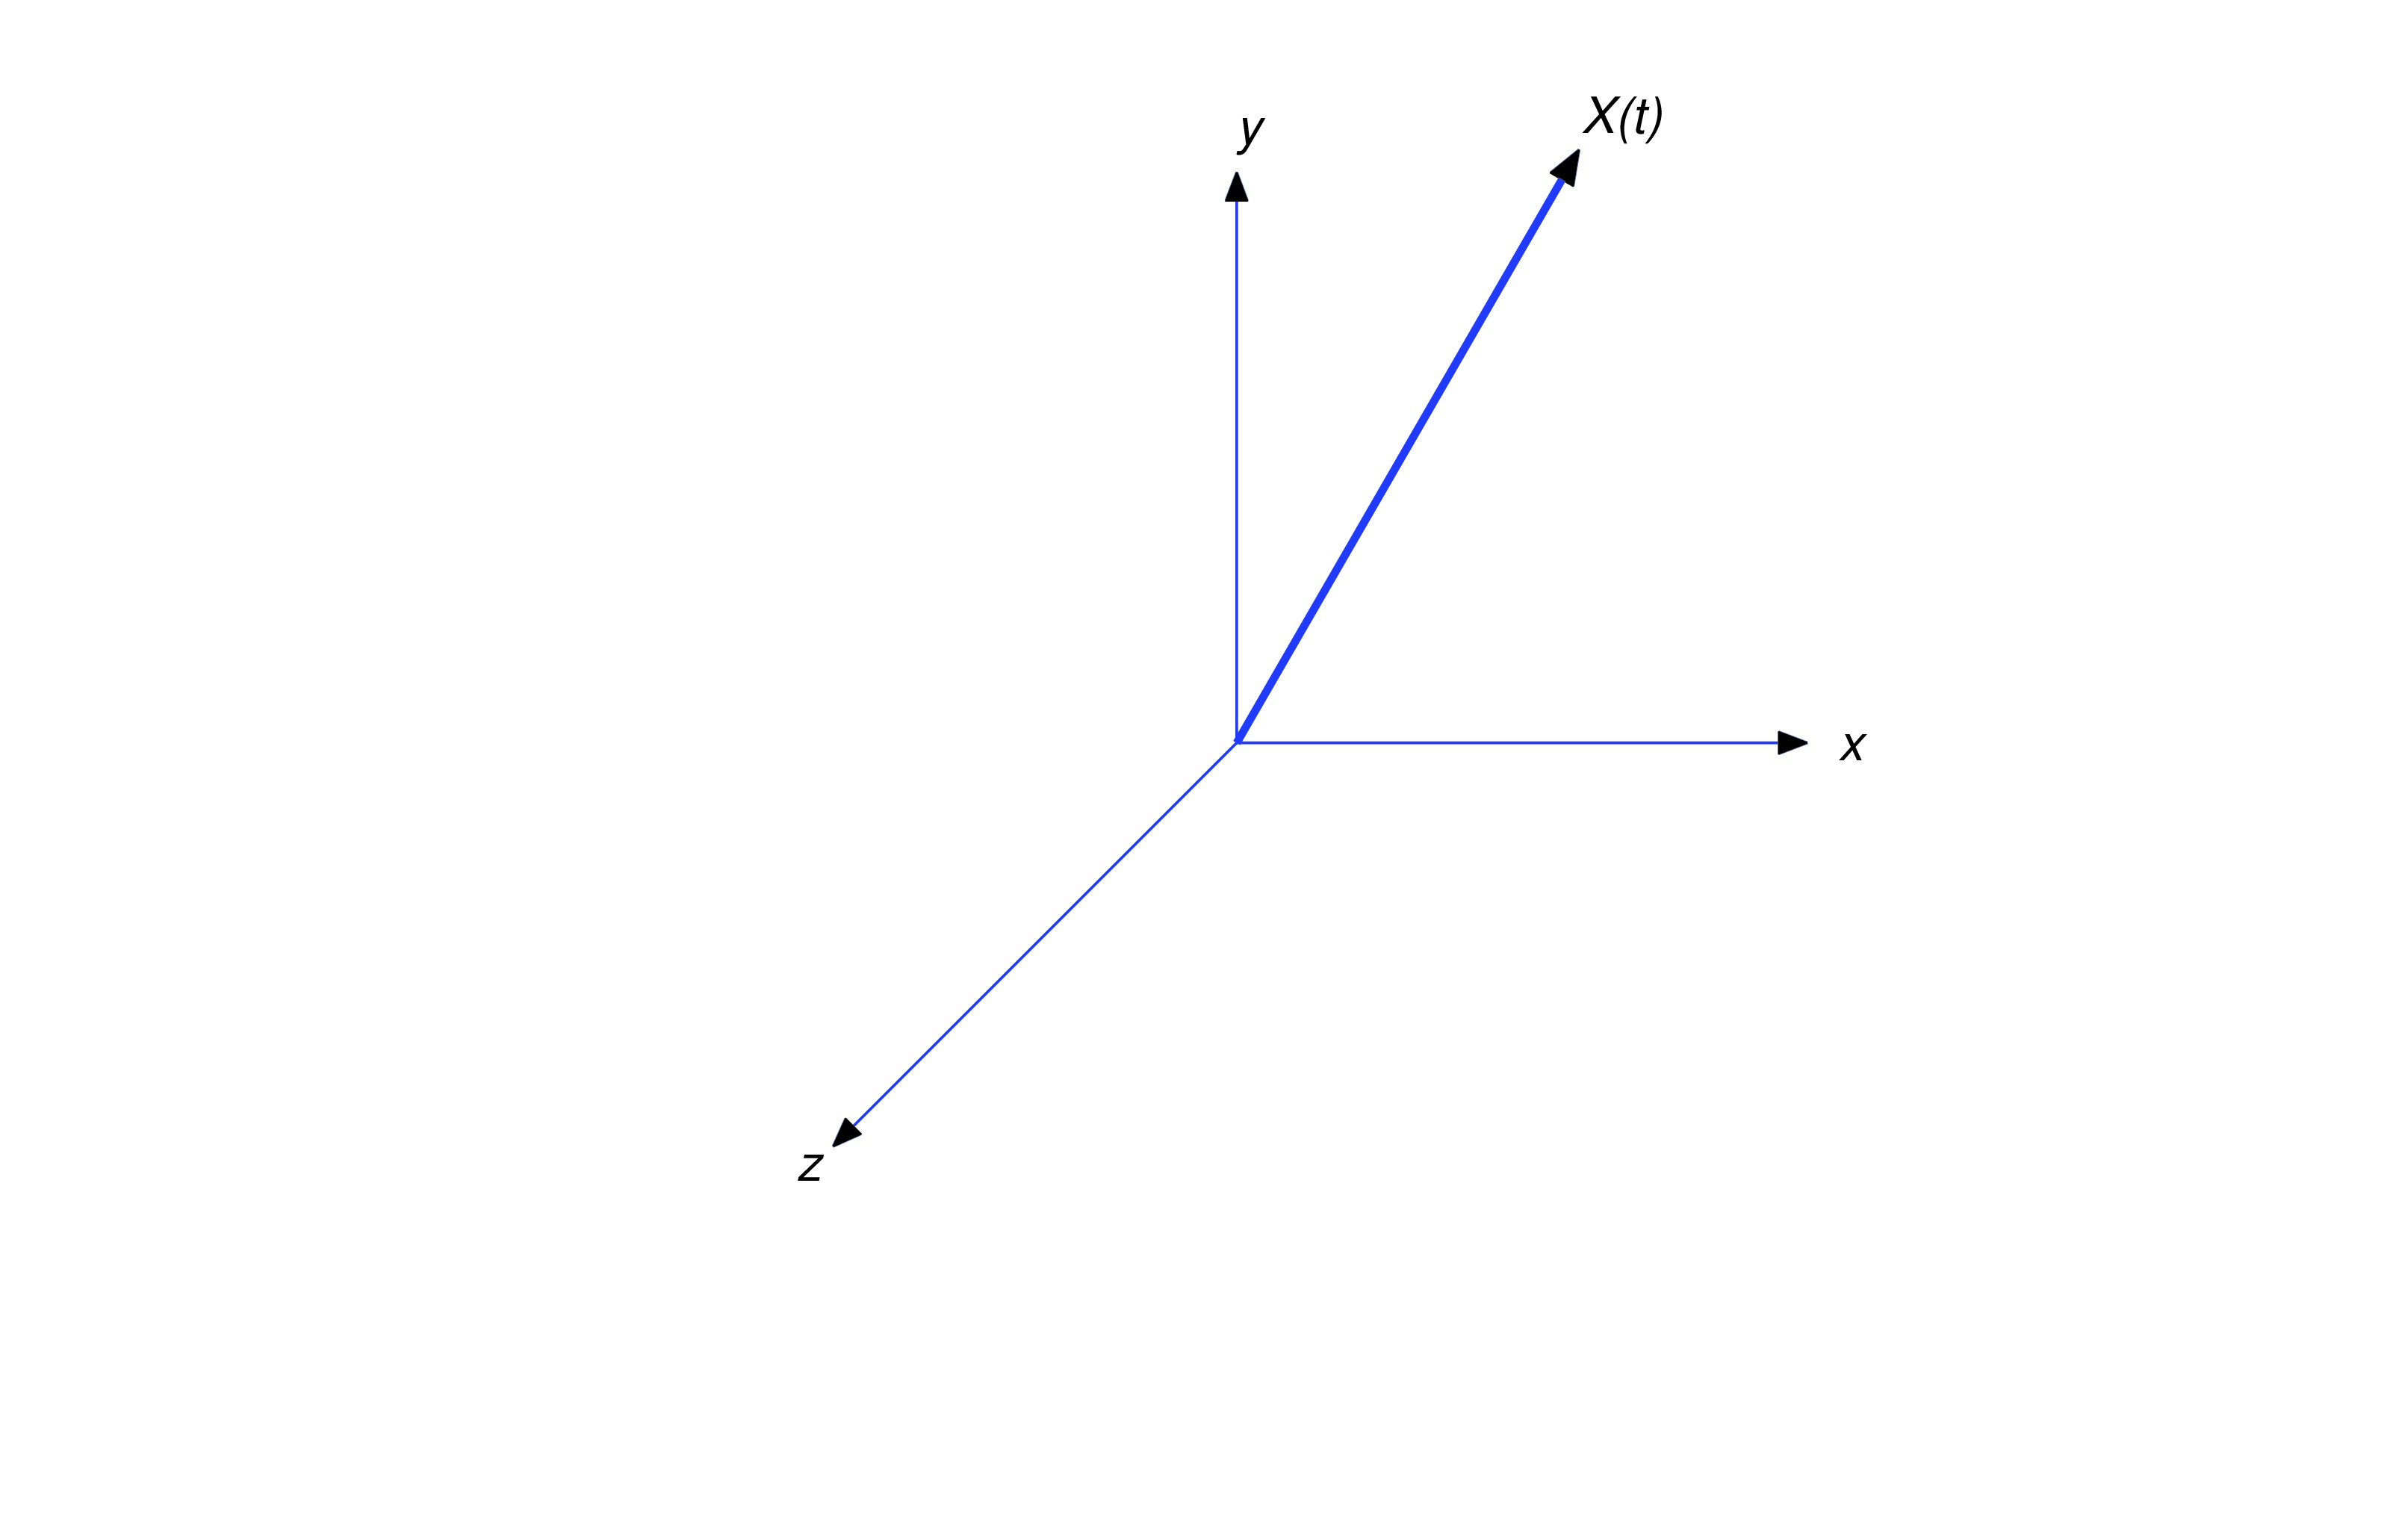
\includegraphics[height=1.5in]{fig100103.jpg} 
\end{image}

According to Newton's law of gravitation,
Earth's gravitational force $\vec{F}=\vec{F}(x,y,z)$ on the object is
inversely proportional to the square of the distance of the object
from Earth's center, and directed toward the center;   thus,
\begin{equation} \label{eq:10.1.13}
\vec{F}=\frac{K}{\norm{\vec{X}}^2}\left(-\frac{\vec{X}}
{\norm{\vec{X}}}\right)=-K\frac{x\,\vec{i}+y\,\vec{j}+z\,\vec{k}}{\left(x^2+y^2+z^2\right)^{3/2}},
\end{equation}
where $K$ is a constant.  To determine $K$,  we observe that the magnitude
of $\vec{F}$  is
$$
\norm{\vec{F}}=K\frac{\norm{\vec{X}}}{\norm{\vec{X}}^3}=\frac{K}{\norm{\vec{X}}^2}
=\frac{K}{(x^2+y^2+z^2)}.
$$
Let $R$  be Earth's radius.
Since $\norm{\vec{F}}=mg$ when the object is at Earth's
surface,
$$
mg = \frac{K}{R^2},\quad\mbox{so}\quad K=mgR^2.
$$
Therefore we can rewrite \eqref{eq:10.1.13} as
$$
\vec{F}=-mgR^2\frac{x\,\vec{i}+y\,\vec{j}+z\,\vec{k}}{\left(x^2+y^2+z^2\right)^{3/2}}.
$$
Now suppose $\vec{F}$ is the only force acting on the object.
According to Newton's second law of motion, $\vec{F}=m\vec{X}''$;   that
is,
$$
 m(x''\,\vec{i}+y''\,\vec{j}+z''\,\vec{k})=
-mgR^2\frac{x\,\vec{i}+y\,\vec{j}+z\,\vec{k}}{\left(x^2+y^2+z^2\right)^{3/2}}.
$$
Cancelling the common factor $m$ and equating components on the two sides
of this equation yields the  system
\begin{equation} \label{eq:10.1.14}
\begin{array}{rcl}
 x''&=&-\frac{gR^2x}{(x^2+y^2+z^2)^{3/2}}\\
 y''&=&-\frac{gR^2y}{(x^2+y^2+z^2)^{3/2}}\\
 z''&=&-\frac{gR^2z}{(x^2+y^2+z^2)^{3/2}}.
\end{array}
\end{equation}
\end{example}

\subsection*{Rewriting Higher Order  Systems as First Order Systems}

A system of the form
\begin{equation} \label{eq:10.1.15}
\begin{array}{ccl}
y_1'&=&g_1(t,y_1,y_2,\dots,y_n)\\
y_2'&=&g_2(t,y_1,y_2,\dots,y_n)\\
&\vdots&\\
y_n'&=&g_n(t,y_1,y_2,\dots,y_n)
\end{array}
\end{equation}
is called a \dfn{first order system}, since the only derivatives
occurring in it are first derivatives. The derivative of
each of the unknowns may depend upon the independent variable and all
the unknowns, but not on the derivatives of other unknowns. When we
wish to emphasize the number of unknown functions in \eqref{eq:10.1.15} we
will say that \eqref{eq:10.1.15} is an $n\times n$ system.

Systems involving higher order derivatives can often be reformulated
as first order systems by introducing additional unknowns. The next
two examples illustrate this.

\begin{example}\label{example:10.1.4}
Rewrite the system
\begin{equation} \label{eq:10.1.16}
\begin{array}{rcl}
m_1y_1''&=&-(c_1+c_2)y_1'+c_2y_2'-(k_1+k_2)y_1+k_2y_2+F_1\\
m_2y_2''&=&c_2y_1'-c_2y_2'+k_2y_1-k_2y_2+F_2.
\end{array}
\end{equation}
derived in Example~\ref{example:10.1.2}  as a system of first order
equations.

\begin{explanation}
If we define $v_1=y_1'$ and $v_2=y_2'$,  then $v_1'=y_1''$ and
$v_2'=y_2''$,  so \eqref{eq:10.1.16} becomes
$$
\begin{array}{rcl}
m_1v_1'&=&-(c_1+c_2)v_1+c_2v_2-(k_1+k_2)y_1+k_2y_2+F_1\\
m_2v_2'&=&c_2v_1-c_2v_2+k_2y_1-k_2y_2+F_2.
\end{array}
$$
Therefore $\{y_1,y_2,v_1,v_2\}$  satisfies the $4\times4$ first order
system
\begin{equation} \label{eq:10.1.17}
\begin{array}{rcl}
y_1'&=&v_1\\
y_2'&=&v_2\\
v_1'&=&\frac{1}{m_1}\left[-(c_1+c_2)v_1+c_2v_2-(k_1+k_2)y_1+k_2y_2+F_1\right]\\
v_2'&=&\frac{1}{m_2}\left[c_2v_1-c_2v_2+k_2y_1-k_2y_2+F_2\right].
 \end{array}
\end{equation}
\end{explanation}
\end{example}


\begin{remark} The difference in form between \eqref{eq:10.1.15} and
\eqref{eq:10.1.17}, due to the way in which the unknowns are \dfn{denoted}
in the two systems, isn't  important;     \eqref{eq:10.1.17} is a first
order system, in that each equation in \eqref{eq:10.1.17} expresses the
first derivative of one of the unknown functions in a way that does
not involve derivatives of any of the other unknowns.
\end{remark}

\begin{example}\label{example:10.1.5}
 Rewrite the system
$$
\begin{array}{ccc} x''&=&f(t,x,x',y,y',y'')\\
y'''&=&g(t,x,x',y,y'y'')
\end{array}
$$
 as a first order system.


\begin{explanation}
We regard $x$, $x'$, $y$, $y'$, and $y''$ as unknown functions, and
rename them
$$
x=x_1,\quad x'=x_2,\quad y=y_1,\quad y'=y_2,\quad y''=y_3.
$$
These unknowns satisfy the system
$$
\begin{array}{ccl} 
x_1'&=&x_2\\
x_2'&=&f(t,x_1,x_2,y_1,y_2,y_3)\\
y_1'&=&y_2\\
y_2'&=&y_3\\
y_3'&=&g(t,x_1,x_2,y_1,y_2,y_3).\end{array}
$$
\end{explanation}
\end{example}

\subsection*{Rewriting Scalar Differential Equations as Systems}

In this chapter we'll refer to differential equations involving only
one unknown function as \dfn{scalar} differential equations. Scalar
differential equations can be rewritten as systems of first order
equations by the method illustrated in the next two examples.

\begin{example}\label{example:10.1.6}
Rewrite the equation
\begin{equation} \label{eq:10.1.18}
y^{(4)}+4y'''+6y''+4y'+y=0
\end{equation}
as a $4\times4$ first order system.

\begin{explanation}
We regard $y$, $y'$, $y''$, and $y'''$  as unknowns and rename them
$$
y=y_1,\quad y'=y_2,\quad y''=y_3,\quad\mbox{and}\quad y'''=y_4.
$$
Then $y^{(4)}=y_4'$, so \eqref{eq:10.1.18} can be written as
$$
y_4'+4y_4+6y_3+4y_2+y_1=0.
$$
Therefore $\{y_1,y_2,y_3,y_4\}$ satisfies the system
 \begin{eqnarray*}
y_1'&=&y_2\\
y_2'&=&y_3 \\
y_3'&=&y_4\\
y_4'&=&-4y_4-6y_3-4y_2-y_1
\end{eqnarray*}
\end{explanation}
\end{example}

\begin{example}\label{example:10.1.7}
 Rewrite
$$
x'''=f(t,x,x',x'')
$$
as a system of first order equations.

\begin{explanation}
We regard $x$, $x'$, and $x''$ as unknowns and rename them
$$
x=y_1, \quad x'=y_2,\quad\mbox{and}\quad x''=y_3.
$$
Then
$$
y_1'=x'=y_2,\quad y_2'=x''=y_3,\quad\mbox{and}\quad y_3'=x'''.
$$
Therefore $\{y_1,y_2,y_3\}$ satisfies the first order system
$$
\begin{array}{ccl}
y_1'&=&y_2\\
y_2'&=&y_3\\
y_3'&=&f(t,y_1,y_2,y_3).
\end{array}
$$
\end{explanation}
\end{example}

Since systems of differential equations involving higher derivatives
can be rewritten as first order systems by the method used in
Examples~\ref{example:10.1.5} --\ref{example:10.1.7} , we'll consider only first
order systems.

\subsection*{Numerical Solution of Systems}

The  numerical methods that we studied in
Chapter~3
can be extended to systems, and most differential equation software
packages include programs to solve systems of equations. We won't go
into detail on numerical methods for systems;     however, for
illustrative purposes we'll describe  the Runge-Kutta method for
the numerical solution of  the initial value problem
\begin{eqnarray*}
y_1'&=&g_1(t,y_1,y_2),\quad y_1(t_0)=y_{10},\\
y_2'&=&g_2(t,y_1,y_2),\quad y_2(t_0)=y_{20}
\end{eqnarray*}
at equally spaced points $t_0, t_1, \dots, t_n=b$ in an interval
$[t_0,b]$. Thus,
$$
t_i=t_0+ih,\quad i=0,1,\dots,n,
$$
where
$$
h=\frac{b-t_0}{n}.
$$
We'll denote the approximate values of $y_1$ and $y_2$ at these
points
by $y_{10},y_{11},\dots,y_{1n}$ and
 $y_{20},y_{21},\dots,y_{2n}$.
The Runge-Kutta method computes these approximate values as follows:
given $y_{1i}$ and $y_{2i}$, compute
\begin{eqnarray*}
I_{1i}&=&g_1(t_i,y_{1i},y_{2i}),\\
J_{1i}&=&g_2(t_i,y_{1i},y_{2i}),\\
I_{2i}&=&g_1\left(t_i+\frac{h}{2},y_{1i}+\frac{h}{2}I_{1i},y_{2i}+\frac{h}{2}J_{1i}\right),\\
J_{2i}&=&g_2\left(t_i+\frac{h}{2},y_{1i}+\frac{h}{2}I_{1i},y_{2i}+\frac{h}{2}J_{1i}\right),\\
I_{3i}&=&g_1\left(t_i+\frac{h}{2},y_{1i}+\frac{h}{2}I_{2i},y_{2i}+\frac{h}{2}J_{2i}\right),\\
J_{3i}&=&g_2\left(t_i+\frac{h}{2},y_{1i}+\frac{h}{2}I_{2i},y_{2i}+\frac{h}{2}J_{2i}\right),\\
I_{4i}&=&g_1(t_i+h,y_{1i}+hI_{3i},y_{2i}+hJ_{3i}),\\
J_{4i}&=&g_2(t_i+h,y_{1i}+hI_{3i},y_{2i}+hJ_{3i}),
\end{eqnarray*}
and
\begin{eqnarray*}
y_{1,i+1}&=&y_{1i}+\frac{h}{6}(I_{1i}+2I_{2i}+2I_{3i}+I_{4i}),\\
y_{2,i+1}&=&y_{2i}+\frac{h}{6}(J_{1i}+2J_{2i}+2J_{3i}+J_{4i})
\end{eqnarray*}
for $i=0, \dots, n-1$. Under appropriate conditions on $g_1$ and $g_2$,
it can be shown that the global truncation error for the Runge-Kutta
method is $O(h^4)$, as in the scalar case considered in
Section~3.3.



\section*{Text Source}
Trench, William F., "Elementary Differential Equations" (2013). Faculty Authored and Edited Books \& CDs. 8. (CC-BY-NC-SA)

\href{https://digitalcommons.trinity.edu/mono/8/}{https://digitalcommons.trinity.edu/mono/8/}


\end{document}